%\newpage
\chapter{Ulteriori Considerazioni sulla Profilatura delle Camme
}\label{cam2}

\section{Una Propriet\`a del Diagramma delle Accelerazioni}

\noindent Vista l'importanza che il diagramma delle accelerazioni riveste nel progetto
dei meccanismi, ci preme mettere in evidenza una sua propriet\`a,
derivante 
da una condizione sussistente nella stagrande maggioranza dei casi
nell'ambito delle camme:
la velocit\`a del cedente deve annullarsi in corrispondenza
dell'inizio ($t=0$) e della fine ($t=t_s$) dell'intervallo di avanzamento.
Si avr\`a quindi
\begin{equation}
\int_0^{t_s} \ddot y\, {\rm d} t = \big|\,\dot y\, \big|_0^{t_s} = 0\,.
\label{e9_risult}
\end{equation}
\noindent L'integrale \ref{e9_risult} evidenzia il fatto che la funzione $\ddot y(t)$ deve avere valor medio
nullo. Svolgiamo ora il seguente integrale, per parti
\begin{equation}
\int_0^{t_s} \ddot y\,t\,{\rm d} t = \big|\,\dot y t\,\big|_0^{t_s} -
\int_0^{t_s} \dot y\,{\rm d} t = 0 - \big|\,y\, \big|_0^{t_s} = -h\,.
\label{e9_moment}
\end{equation}

\begin{figure}[b]
\setlength{\unitlength}{1mm}
\centerline{
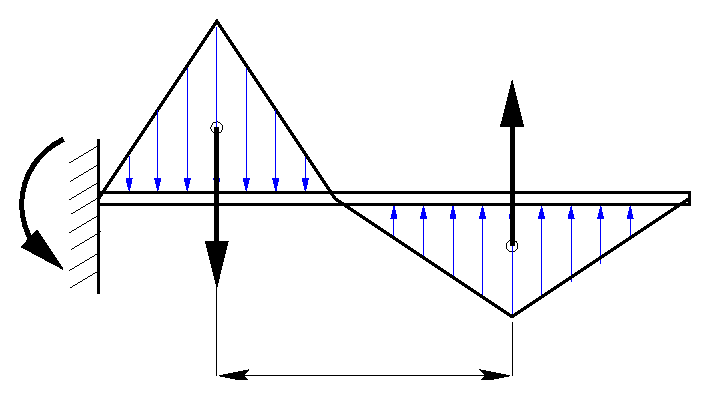
\epsfig{file=part3/camme/FIG/trave.eps,height=3cm}
}
\begin{picture}(0,0)(-30,0)
\scriptsize{
\put( 1,20){$M_i$}
\put(33, 7){d}
\put(48,29){$\dot y_{max}$} 
\put(23,13){$\dot y_{max}$} 
}
\end{picture}
\vskip -5mm
\caption
{
{\em Analogia fra diagramma delle accelerazioni e diagramma dei carichi.}
\label{f9_trave}
}
\end{figure}
\noindent Le relazioni \ref{e9_moment} assumono particolare evidenza alla luce della seguente
analogia: immaginando il diagramma delle accelerazioni $\ddot y$ come quello
di un carico distribuito lungo una trave incastrata a un estremo e di
lunghezza $t_s$, le precedenti relazioni equivalgono, in tal caso,
a imporre che tale carico
debba avere risultante nulla e momento all'incastro $M_i=h$.

\section{Un Metodo per Ridurre l'Ingombro delle Camme}\index{camme!offset}\index{camme}

\noindent Come \`e stato esposto a pagina \pageref{fig:f_ang_press}, l'angolo di pressione
massimo costituisce spesso un limite gravoso nel progetto  di una camma,
costringendo il progettista ad aumentare le dimensioni dell'eccentrico,
e spesso anche quelle della macchina, onde evitare gli
inconvenienti dovuti alle elevate forze laterali che nascono e i conseguenti
pericoli di impuntamento.

\begin{figure}[hbt]
\begin{center}
\hbox{\vspace{.5cm}\hspace{-1cm}\includegraphics[width=.9\textwidth]{part3/camme/FIG/camma/camma_offset.pdf}}
\vspace{-4cm}\hspace{7.5cm}\includegraphics[width=0.3\textwidth]{part3/camme/FIG/camma/camma_offset_ruotata.pdf}
\end{center}
\begin{picture}(0,0)(-20,-20)
\scriptsize{
\put(40,223){${\rho}_{\rm min}=24.4\; {\rm mm,\;}\;\alpha=119^{\circ}$}
\put(57,220){\rotatebox{-61}{$\rightarrow$}}
\put(93,217){\rotatebox{-77}{$\rightarrow$}}
\put(98,213){$\theta_{\rm max}=27^{\circ},\; \alpha=103^{\circ}$}
\put(226,98){$R_b=80.1\,{\rm mm}$}
\put(95,130){$\epsilon= 13\, {\rm mm}$}

\put(175,0){meccanismo ruotato di$\;\;\xi=-\arcsin({\frac{\epsilon}{R_b}})$}
}
\end{picture}
      \caption{\em Camma con punteria deviata.}
 \label{fig:camma_offset}
\end{figure}

\noindent Va detto per\`o che, mentre il contenimento di $\theta_{\rm max}$, nelle
fasi di lavoro (di solito chiamate salite),
deriva dalle cautele atte a  evitare una trasmissione
inefficiente delle forze, pericoli di impuntamenti e reazioni vincolari eccessive,
tali precauzioni si possono lasciare cadere 
nei tratti di riposo della camma, cio\`e nelle fasi  di discesa.
Pertanto, se inclinassimo il cedente in modo da diminuire l'angolo di pressione 
nelle fasi di salita, potremmo tollerare l'aumento di $\theta$
nelle fasi in cui tale cedente \`e scarico.
In figura \ref{fig:camma_offset} \`e riportata una camma tastata da un cedente a punteria con
rotella. Per inciso, tale camma \`e la stessa di figura
\ref{fig:f_camma_rotella}, dove per\`o il cedente
\`e disassato di una quantit\`a $\epsilon= 13\,{\rm mm}$ rispetto al centro
della camma stessa\footnote{Si \`e preferito lasciare inalterata la distanza del centro della rotella rispetto al centro della camma
in direzione orizzontale, che risultava essere
$80\,{\rm mm}$; per tale motivo il raggio di base attuale risulta leggermente pi\`u grande.}.
In basso a destra, nella stessa figura, mostriamo il medesimo meccanismo
ruotato di $\xi=9.34^{\circ}$, che dovrebbe mettere in luce la sostanziale
equivalenza della punteria deviata
con la scelta, per il suo movimento, di una direzione inclinata rispetto alle
 alzate fornite dalla sagoma di traslazione, cio\`e dalla legge delle alzate.
Per la precisione,
 l'angolo $\xi$ \`e variabile dovendo essere
$\sin\xi(\alpha)=\epsilon / (R_b + h(\alpha))$, dove $h(\alpha)$
\`e, come sempre, l'alzata all'angolo $\alpha$.
Utilizzando quindi il {\em cedente deviato}\index{cedente!deviato},
i valori di $\theta_{\rm max}$
 differiscono di poco meno di $7^{\circ}$,
 come si pu\`o notare osservando le figure \ref{fig:f_camma_rotella} e
 \ref{fig:camma_offset};
tale differenza
ci permetter\`a, come vedremo a breve, di diminuire l'ingombro della camma.
Per maggiore chiarezza, in figura \ref{fig:ap_offset} sono
riportati i grafici dell'angolo di pressione della camma con
cedente centrato unitamente a quello della
camma con punteria deviata, e la differenza tra i due varia
tra valori di poco inferiori a
$7^{\circ}$ e valori di poco superiori a $9^{\circ}$.

\begin{figure}[hbt]
\begin{center}
\includegraphics[width=0.7\textwidth]{part3/camme/FIG/camma/ap_offset.pdf}
\end{center}
\begin{picture}(0,0)(-150,0)
\scriptsize{
\put(15,108){rotella in asse}
\put(15,80){rotella {\em offset}}
}
\end{picture}
\vskip -5mm
      \caption{\em Confronto tra gli angoli di pressione.}
 \label{fig:ap_offset}
\end{figure}
\noindent Ancora dalla figura \ref{fig:ap_offset}
apprendiamo che l'{\em escamotage} della soluzione {\em offset} si
ripercuote in modo negativo sull'angolo di pressione non solo 
nelle fasi di discesa, ma anche nelle soste, cio\`e quando il profilo della
camma \`e circolare. Mentre il valore assunto da $\theta$ durante le 
discese \`e in generale indifferente, dobbiamo considerare che spesso,
durante le soste, la camma sta esercitando il valore massimo della forza
(situazione tipica nelle presse), quindi un valore di $\theta$ diverso
da zero in queste fasi va attentamente valutato.
Ciononostante, i benefici tecnici che si ottengono con la riduzione
dell'ingombro della
camma, quindi dell'intero corpo della macchina, mediante disassamento del cedente vengono sovente ritenuti irrinunciabili.
Tale riduzione delle dimensioni della camma si opera naturalmente
ridimensionando il raggio di 
base nella soluzione {\em offset} fino a che uno dei due limiti
costituiti dall'angolo di pressione massimo e dal minimo raggio di curvatura 
convessa non viene raggiunto.
La figura \ref{fig:camma_offset_ottimizzata} riporta tale compromesso:
$\theta_{\rm max}=31^{\circ}$ e $\rho_{\rm min}=13\, {\rm mm}$.
Questi due valori offrono sufficienti garanzie per il buon
funzionamento del meccanismo e la camma che li esprime ha un
raggio di base ridotto del 25\% rispetto a quella non ottimizzata.
Quest'ultima \`e presente nella figura in colore tenue.

\begin{figure}[hbt]
\centering
\begin{minipage}[b]{0.6\textwidth}
\centering
\begin{center}
\includegraphics[width=0.9\textwidth]{part3/camme/FIG/camma/camma_offset_ottimizzata.pdf}
\end{center}
\begin{picture}(0,0)(65,0)
\scriptsize{
\put(5,170){${\rho}_{\rm min}=13\; {\rm mm,\;}\;\alpha=121^{\circ}$}
\put(13,166){\rotatebox{-59}{$\longrightarrow$}}
\put(38,157){\rotatebox{-77}{$\rightarrow$}}
\put(44,154){$\theta_{\rm max}=31^{\circ},\; \alpha=103^{\circ}$}
}
\end{picture}
      \caption{\em Camma {\em offset} con ingombro ridotto.}
 \label{fig:camma_offset_ottimizzata}
\end{minipage}\hfill
\begin{minipage}[b]{0.38\textwidth}
\centering
\hbox{\vspace{1cm}\includegraphics[width=0.9\textwidth]{part3/camme/FIG/camma/ap_offset_ottimizzata.pdf}}
\begin{picture}(0,0)(100,0)
	\scriptsize{
\put(77,93){\tiny non ottimizzata (rosa)}
\put(45,66){\tiny ottimizzata (verde)}
\put(152,43){$\alpha$}
}
\end{picture}
	\caption{\em Confronto tra gli angoli di pressione prima e dopo l'ottimizzazione.}
     \label{fig:ap_ottimizzata}
\end{minipage}
\end{figure}

\noindent Stiamo via via approcciando la soluzione tecnica ottimale
della profilatura delle camme che entrano nel progetto di una pressa.
Occorre ora pensare alla camma coniugata o
desmodromica che dovr\`a garantire il ritorno della mazza.
La figura \ref{fig:camma_ood} riporta il gruppo camma primaria, camma coniugata
e il telaio dei cedenti con le relative rotelle. Si pu\`o notare che la soluzione {\em offset} interessa anche la camma desmodromica che presenta, laddove
si trova impegnata nel ritorno della punteria, angoli di pressione modesti,
come mostrato in figura \ref{fig:ap_ood}.
La figura \ref{fig:camma_ood} evidenzia anche
due caratteristiche particolari della camma desmodromica: un raggio di curvatura
eccessivamente ridotto e un angolo di pressione troppo elevato.
Tale circostanza per\`o non
desta alcun timore, presentandosi in zone dove l'eccentrico non \`e impegnato
da alcuna forza\footnote{Il gruppo desmodromico di figura \ref{fig:camma_ood}
\`e stato prodotto in quattro esemplari. Le otto camme di spessore pari a
$25\, {\rm mm}$ sono state ritagliate, tramite una macchina a {\em
elettroerosione a filo} e controllo numerico, direttamente da una lastra di
acciaio 35 NiCrMo 15, gi\`a bonificato. Esse azionano due piccole presse la cui
forza \`e pari a circa una tonnellata.}.
\begin{figure}[b]
\centering
\begin{minipage}[b]{0.6\textwidth}
\centering
\begin{center}
\includegraphics[width=0.9\textwidth]{part3/camme/FIG/camma/camma_ood.pdf}
\end{center}
\begin{picture}(0,0)(65,0)
\scriptsize{
\put(47,20){${\rho_c}_{\rm min}=1.4\; {\rm mm,\;}\;\alpha=274^{\circ}$}
\put(52,27.3){\rotatebox{94}{$\longrightarrow$}}
\put(63,50){\rotatebox{112}{$\rightarrow$}}
\put(62,38){$\theta_{\rm max}=57^{\circ},\;\; \alpha=291^{\circ}$}
}
\end{picture}
      \caption{\em Gruppo camma-desmodromica ottimizzato.}
 \label{fig:camma_ood}
\end{minipage}\hfill
\begin{minipage}[b]{0.38\textwidth}
\centering
\hbox{\vspace{1cm}\includegraphics[width=0.90\textwidth]{part3/camme/FIG/camma/ap_ood.pdf}}
\begin{picture}(0,0)(100,0)
	\scriptsize{
\put(82,89){\tiny coniugata}
\put(62,64){\tiny primaria}
\put(155,43){$\alpha$}
}
\end{picture}
	\caption{\em Confronto tra gli angoli di pressione.}
     \label{fig:ap_ood}
\end{minipage}
\end{figure}

\section{Cenni alla Profilatura di Camme con Cedente a Bilanciere}

\noindent Come accennato a pagina \pageref{fig:f_cambil}, il cedente
a punteria traslante viene talvolta sostituito
da un bilanciere che, anzich\'e traslare, ruota.
Questa soluzione tecnica offre il vantaggio costruttivo di eliminare 
le guide di scorrimento della punteria e di offrire in modo nativo
l'opportunit\`a di posizionare, in cascata all'azionamento a camma,
un sistema articolato, spesso
un manovellismo, la cui manovella pu\`o essere  costituita direttamente
dal bilanciere che tasta la camma.
\`E evidente che, a valle del manovellismo o del quadrilatero azionato
tramite un cedente a bilanciere, otterremo delle leggi di moto diverse
rispetto a quelle implementate sulla camma stessa.
La qual cosa non deve apparire in una luce negativa. Spesso infatti il
sistema articolato posto in serie all'azionamento a camma favorisce
l'ottenimento di una legge delle alzate che soddisfa ancora meglio le
esigenze del processo tecnologico che d\`a origine al progetto.
Entrare nel merito della progettazione di un sistema complesso, come pu\`o
essere un sistema articolato azionato da una camma, esula completamente
dallo scopo di questo lavoro. Segnaliamo solo che la maggior parte
dei programmi di calcolo commerciali che assistono il progettista di 
meccanismi permette di affrontare questo tipo di analisi.

\noindent Torniamo quindi alla nostra camma a bilanciere\index{camme!a bilanciere},
consapevoli di esporre un argomento ``zoppo'', in quanto molto difficilmente
il tema assegnato consiste solo nella rotazione di un bilanciere sia pure 
con leggi ben precise. 
In questo caso, la legge di moto $\beta(\alpha)$ riguarder\`a la rotazione del
bilanciere a partire dalla sua configurazione di riposo.
Giusto per fornire un'idea del percorso di progetto per questo tipo di camma
abbiamo confezionato una legge di moto tale che, applicata alle rotazioni
del bilanciere, non produce movimenti della rotella troppo dissimili rispetto
alla legge delle alzate di figura \ref{fig:f_legge_completa_7_h}
se non
per la natura diversa dei suoi spostamenti, che in questo
caso seguono traiettorie circolari
anzich\'e rettilinee. Il risultato della sintesi di tale camma (e della sua
coniugata) \`e riportato in figura \ref{fig:camma_bilanciere}.

\begin{figure}[hbt]
\centering
\includegraphics[width=0.9\textwidth]{part3/camme/FIG/camma/camma_bilanciere_desmo.pdf}
\begin{picture}(0,0)(150,-20)
\scriptsize{
}
\put(51,260){\rotatebox{-155}{$\curvearrowleft$}}
\put(62,256){$\beta(\alpha)$}
\put(84.5,180){$\beta_{\rm max}= 24^{\circ}$}
\put(88,220){$l= 85 {\rm mm}$}
%\put(-25,150){$\curvearrowright$}
%\put(-25,155){$\omega$}
\put(76,85){$R_b=50 {\rm mm}$}
\end{picture}
        \caption{\em Camma desmodromica con cedente a bilanciere.}
     \label{fig:camma_bilanciere}
\end{figure}

\noindent La figura \ref{fig:legge_camma_bilanciere} mostra la legge di
$\beta(\alpha)$ e quella di accelerazione $\beta''(\alpha)$, espresse rispettivamente
in gradi sessagesimali e gradi sessagesimali  su gradi radianti al quadrato.
L'azionamento della camma comporta dunque un movimento oscillatorio del
bilanciere che spazia in un arco di
$24^{\circ}$. Tale oscillazione consente alla rotella di tracciare un arco di circa $40 \,{\rm mm}$
tastando una camma avente raggio di base $R_b=50\,{\rm mm}$ tramite un bilanciere
di lunghezza $l=85\, {\rm mm}$, il che equivale all'incirca all'azionamento
operato dalla camma di figura \ref{fig:f_camma_rotella} con ingombro leggermente
pi\`u contenuto.
Naturalmente \`e quasi sempre necessario, anche per le camme a bilanciere,
progettare la camma coniugata che permette il cosiddetto {\em positive
drive}, cio\`e l'azionamento sempre condotto da forze di pressione positive.
Come abbiamo gi\`a accennato, la figura \ref{fig:camma_bilanciere} riporta
anche la camma coniugata e il relativo bilanciere.
I due bilancieri, che devono essere considerati come un unico corpo rigido,
sono rappresentati con tinte pi\`u tenui anche nelle due posizioni di sosta,
appena a valle delle due alzate prodotte dalla legge di moto.

\begin{figure}[hbt]
\centering
\includegraphics[width=0.7\textwidth]{part3/camme/FIG/camma/legge_camma_bilanciere.pdf}
\begin{picture}(0,0)(150,-20)
\put(15,91){$\beta(\alpha)$}
\put(15,67){$\beta''(\alpha)$}
\put(133,-13.5){$\alpha$}
\end{picture}
        \caption{\em Leggi di moto del bilanciere.}
     \label{fig:legge_camma_bilanciere}
\end{figure}

\noindent Mentre le cautele che riguardano il raggio di curvatura
minimo del profilo nella parte convessa rimangono fondamentali anche per
queste camme, le restrizioni che riguardano l'angolo di pressione sono
in generale pi\`u lasche. Il motivo di questa maggiore tolleranza,
soprattutto quando la camma, girando come di consueto in senso
orario, \`e disposta rispetto al cedente a bilanciere nella configurazione
riportata in figura, cio\`e quando la camma viene ``accarezzata dal cedente'', 
risiede nella
notevole diminuzione del pericolo di impuntamento e di scarso rendimento che si
verifica
nelle guide di scorrimento di punterie impegnate da notevoli azioni
laterali. Rimane tuttavia da considerare l'inefficienza di trasmettere
forze fuori asse rispetto alla direzione del moto. 

\section{Cenni alla Profilatura di Camme Tastate da Piattello}\index{camme!cedente a piattello}

\noindent Come gi\`a accennato a pagina \pageref{fig:f_campiat}, si trova
nella tecnica una vasta famiglia di camme tastate da un cedente
che striscia mediante una porzione di superficie, generalmente
piana, sul profilo della camma
stessa: le camme tastate da piattello. Queste camme popolano il mondo
dell'{\em automotive} essendo normalmente responsabili dell'apertura e della
chiusura dei condotti di aspirazione e di scarico dei gas nei motori a quattro
tempi. Il loro ingombro raramente eccede i $40\, {\rm mm}$; il cedente
 pu\`o essere
una punteria traslante oppure un bilanciere e il contatto tra camma e cedente
\`e quasi sempre garantito da una molla pre-caricata, anche se esistono esempi
notevoli di azionamenti a camme, per valvole di motori endotermici, di
tipo desmodromico.
Il percorso che abbiamo seguito per la sintesi delle camme tastate da rotella
rimane valido anche in quest'ambito bench\'e non sempre i progettisti di camme
per motori partono dalla legge dell'accelerazione. Quest'ultima rimane comunque
una caratteristica importantissima dell'azionamento in quanto anche da essa dipendono
i malfunzionamenti del motore ad alti regimi di rotazione; quando cio\`e
le valvole, trascinate dalle loro forze d'inerzia, si staccano dalla camma
nonostante la presenza delle molle, causando il cosiddetto {\em sfarfallamento}\index{sfarfallamento}.
Ciononostante, in ambito motoristico, non \`e infrequente privilegiare
la legge delle alzate partendo nel processo di sintesi da
questa, e verificare a posteriori che essa non produca
accelerazioni inaccettabili.

\noindent Se tentassimo di disegnare una camma per motore a quattro tempi
provvista delle proporzioni geometriche  caratteristiche in questo campo,
ed eseguissimo questo tentativo
adagiando ingenuamente sul tamburo della camma
una legge di moto ottenuta disponendo
in serie un paio delle solite leggi trapezoidali modificate, come quelle di figura
\ref{fig:leggi_camma_piattello_ingenua}\footnote{In
questa e nelle figure analoghe che seguiranno \`e sottintesa la misura delle
accelerazioni in millimetri su secondo quadro, delle velocit\`a
in millimetri al secondo e infine dell'alzata
in millimetri.},
otterremmo il pessimo risultato gi\`a illustrato in figura
\ref{fig:f_sottotaglio} e di nuovo proposto in figura
\ref{fig:camma_piattello_ingenua}.

\begin{figure}[hbt]
\centering
\begin{minipage}[b]{0.48\textwidth}
\centering
\includegraphics[width=0.8\textwidth]{part3/camme/FIG/camma/camma_piattello_ingenua.pdf}
\begin{picture}(0,0)(0,0)
\scriptsize{
}
\end{picture}
      \caption{\em Camma a piattello inservibile.}
 \label{fig:camma_piattello_ingenua}
\end{minipage}\hfill
\begin{minipage}[b]{0.48\textwidth}
\centering
\includegraphics[width=0.8\textwidth]{part3/camme/FIG/camma/leggi_camma_piattello_ingenua.pdf}
\begin{picture}(0,0)(80,0)
	\scriptsize{
\put(-5,70){\color{red}$y''(\alpha)$}
\put(-10,30){\color{dark-green}$y'(\alpha)$}
\put(20,47){\color{blue}$y(\alpha)$}
\put(67,2){$\alpha$}
}
\end{picture}
	\caption{\em Approccio ingenuo alla camma con piattello.}
     \label{fig:leggi_camma_piattello_ingenua}
\end{minipage}
\end{figure}
 
\noindent L'esperimento numerico
\`e stato condotto rispettando i seguenti parametri: raggio della porzione circolare della camma
$R_c=14\,{\rm mm}$\footnote{Ricordiamoci la scelta, operata a suo tempo, di
chiamare raggio di base $R_b$ quello del percorso del centro della rotella. Come
abbiamo detto in altro luogo moltissimi autori chiamano raggio di base quello
della porzione circolare ad alzata zero del profilo fisico. Qui viene indicato
con $R_c$.}, alzata massima $h=12\, {\rm mm}$, angolo di salita
$\alpha_s=75^{\circ}$ e angolo di discesa $\alpha_d=75^{\circ}$.
Questi dati corrispondono all'incirca a quelli delle camme di aspirazione
di un motore Alfa Romeo che equipaggiava la Giulia 1600 cc GTA.
Il marcato sottotaglio, che la figura
\ref{fig:camma_piattello_ingenua} evidenzia,
si spiega pensando il piattello come una rotella di raggio $r_r$ infinito 
che tasta una camma di raggio di base $R_b$ altrettanto infinito dove la 
differenza $R_b - r_r = R_c$. 
\`E opportuno a questo punto ricordare la formula \ref{r_cur} che fornisce
il raggio di curvatura del profilo della camma, una volta sottratto quello
della rotella. Avremo
\begin{equation}
\rho ={{{{[{{y'}^2\over{(R_b + y)^2}}+1]}^{3/2}(R_b+y)}\over{{1-{y''\over{(R_b + y)}}} +{2{y'}^2\over{(R_b + y)^2}}}}}-(R_b-R_c)\,,
\label{r_cur_piat0}
\end{equation}
\noindent quindi per elevati valori di $R_b$
\begin{equation}
\lim_{R_b\to\infty}\rho =
\lim_{R_b\to\infty}{(R_b+y)\over{1 -{y''\over{(R_b + y)}}}} -(R_b-Rc)\,.
\label{r_cur_piat2}
\end{equation}
\noindent Mediante pochi passaggi, che lasciamo al lettore, otteniamo
\begin{equation}
\lim_{R_b\to\infty}\rho =
R_c + y + y''\,,
\label{r_cur_piat1}
\end{equation}
\noindent riportata con altri simboli anche in \cite{ruggieri}, pag. 67.
\noindent Il pericolo di profilo intrecciato si manifester\`a dunque
per valori negativi di $y''$ e, come sempre, tale pericolo
\`e scongiurato dal crescere delle dimensioni della camma, cio\`e di $R_c$.
Occorre quindi ricercare leggi di moto con  bassi valori assoluti di
accelerazione negativa, compatibilmente
con l'esigenza di avere valori non eccessivi di accelerazione positiva.
In figura \ref{fig:acc_piat} \`e rappresentata una legge idonea a ottenere
la camma che stiamo cercando e che rappresentiamo in figura
\ref{fig:camma_piattello}.
Si noti che le due leggi di accelerazione sono profondamente asimmetriche e che
i bassi valori assoluti di accelerazione negativa risultano indispensabili
laddove anche il valore dell'alzata \`e modesto, come si evince facilmente dalla
formula \ref{r_cur_piat1}.

\begin{figure}[hbt]
\centering
\begin{minipage}[b]{0.48\textwidth}
\centering
\includegraphics[width=0.8\textwidth]{part3/camme/FIG/camma/camma_piattello.pdf}
\begin{picture}(0,0)(0,0)
\scriptsize{
}
\end{picture}
      \caption{\em Camma tastata da piattello ottenuta da leggi trapezoidali modificate.}
 \label{fig:camma_piattello}
\end{minipage}\hfill
\begin{minipage}[b]{0.48\textwidth}
\centering
\includegraphics[width=0.8\textwidth]{part3/camme/FIG/camma/leggi_camma_piattello.pdf}
\begin{picture}(0,0)(80,0)
	\scriptsize{
\put(-50,83.6){$y''_{\rm max}=84\,{\rm mm}/{\rm rad}^2$}
\put(-5,70){\color{red}$y''(\alpha)$}
\put(-6,27){\color{dark-green}$y'(\alpha)$}
\put(20,43){\color{blue}$y(\alpha)$}
\put(67,2){$\alpha$}
}
\end{picture}-
	\caption{\em Legge di moto composta da due leggi trapezoidali modificate adatta per camma-piattello.}
     \label{fig:acc_piat}
\end{minipage}
\end{figure}

\noindent 

\noindent Il cedente con piattello non
\`e azionato, in generale, dal punto del profilo che si trova sull'asse del
cedente, perch\'e il contatto tra il profilo stesso e il piattello pu\`o
trovarsi altrove. \`E il caso di avvertire il lettore che per le camme
tastate da piattello l'angolo di pressione \`e sempre costante e, nel solo
caso che abbiamo trattato, vale a dire quello che presenta
l'asse della punteria ortogonale
alla superficie del piattello stesso, risulta essere $\theta=0$.

\noindent Da alcuni rilievi, eseguiti sulla camma della nota casa
automobilistica, possiamo affermare che essa non coincide con quella di 
figura \ref{fig:camma_piattello}, anzi a un occhio appena allenato le
due camme appaiono alquanto difformi.
Ci \`e sembrato cos\`i di qualche interesse eseguire un tentativo numerico 
volto alla interpolazione dei pochi valori rilevati dal profilo della camma
originale e tratti da un
vecchio disegno a nostra disposizione.
Tale interpolazione, svolta tramite {\em spline cubiche}\index{spline},
fornisce il profilo della camma\footnote{Si tratta del profilo effettivo della
camma, cio\`e di una sagoma di traslazione che aggiunta al tamburo della
camma stessa produrr\`a lo stesso contorno dell'eccentrico rilevato dal  disegno
che abbiamo a disposizione.
Questa sagoma di traslazione non coincide pertanto con la legge delle 
alzate del piattello che in seguito riporteremo.} riportato in figura
\ref{fig:spline_profilo_completa}, dove le crocette indicano i pochi punti misurati.

\begin{figure}[hbt]
\begin{center}
\includegraphics[width=0.6\textwidth]{part3/camme/FIG/camma/spline/spline_profilo_completa.pdf}
\end{center}
\begin{picture}(0,0)(-150,0)
\scriptsize{
}
\end{picture}
      \caption{\em {\em Spline} del profilo della camma.}
 \label{fig:spline_profilo_completa}
\end{figure}

\noindent Aggiungendo questa ``finta'' sagoma di traslazione ad un tamburo con
$R_b=14\,{\rm mm}$, comportandoci cio\`e come se la camma dovesse essere in seguito
tastata da una punta, otteniamo la figura \ref{fig:cammaspline}
che mostra un eccentrico praticamente identico a quello
realmente impiegato nella citata automobile.
 
\begin{figure}[hbt]
\centering
\begin{minipage}[b]{0.48\textwidth}
\centering
\includegraphics[width=0.8\textwidth]{part3/camme/FIG/camma/spline/camma_piattello_profilo_spline.pdf}
\begin{picture}(0,0)(0,0)
\scriptsize{
}
\end{picture}
      \caption{\em Camma con profilo ottenuto dalla {\em spline} di fig. \ref{fig:spline_profilo_completa}.}
 \label{fig:cammaspline}
\end{minipage}\hfill
\begin{minipage}[b]{0.48\textwidth}
\centering
\includegraphics[width=0.8\textwidth]{part3/camme/FIG/camma/spline/leggi_piattello_profilo_spline.pdf}
\begin{picture}(0,0)(80,0)
	\scriptsize{
\put(-45,84){$y''_{\rm max}=110\,{\rm mm}/{\rm rad}^2$}
\put(4,70){\color{red}$y''(\alpha)$}
\put(3,28){\color{dark-green}$y'(\alpha)$}
\put(20,45){\color{blue}$y(\alpha)$}
\put(67,2){$\alpha$}
}
\end{picture}
	\caption{\em Effettive leggi di moto.}
     \label{fig:leggi_spline}
\end{minipage}
\end{figure}

\noindent La camma in questione \`e per\`o tastata da un piattello anzich\'e da una
punta. \`E interessante perci\`o ricavare le leggi di moto effettivamente
ottenute, che riportiamo in figura \ref{fig:leggi_spline}. 
Pur riconoscendo in tali leggi molte somiglianze con quelle canoniche di
figura \ref{fig:acc_piat}, prendiamo atto che la loro forma contiene variazioni
impossibili da ottenere
sfruttando solamente le possibilit\`a offerte dalla legge di moto trapezoidale
modificata.
\`E il caso di aggiungere che la corretta lubrificazione gioca un ruolo
fondamentale nelle camme tastate da piattello. Mentre si possono trovare
meccanismi camma-rotella sia immersi in bagno d'olio, sia lubrificati
con maggior superficialit\`a, \`e praticamente impossibile pensare a una
coppia camma-piattello che non sia fornita di lubrificazione forzata
e costante, come effettivamente avviene nei motori a combustione interna
a quattro tempi.
\newpage
\thispagestyle{empty}
\null
\endinput
